\section{Experiments}
\subsection{Comparing Fitting time and performance of FastSRM and
  SRM on synthetic data}
We generate data $\xb_i$ according to the model of Probabilistic SRM. We sample the value of the subject specific noise level from a normal
distribution: $\sigma_i \sim \Ncal(0, 0.1)$. The coefficients of the mixing matrices $A_i$
are obtained by sampling their coefficient from a standardized normal distribution.
Lastly, the covariance of the shared response $\Sigma_s$ is diagonal and the
diagonal values are obtained by sampling from a Dirichlet distribution with
parameter $(1 \dots 1)$.

As the deterministic SRM algorithm is only identifiable up to an arbitrary
rotation we measure the distance between the true component $S \in \RR^{p, n}$ and
the predicted component $\hat{S} \in \RR^{p, n}$ by the quantity:
$min_{A \in \RR^{p, p}} \|A \hat{S} - S \|^2_F =  \|S \hat{S}^{\dagger}\hat{S} - S \|^2_F$.






\subsubsection{Datasets}

We use five fMRI datasets of subjects exposed to naturalistic stimuli. When needed, datasets are preprocessed with FSL \url{http://fsl.fmrib.ox.ac.uk/fsl} using slice time correction, spatial realignment, coregistration to the T1 image and affine transformation of the functional volumes to a template brain (MNI). Using nilearn \cite{abraham2014machine}, preprocessed data are resampled, masked (using a full brain mask available at \url{http://cogspaces.github.io/assets/data/hcp_mask.nii.gz}), detrended and standardized after a 5 mm smoothing is applied.  
%
\paragraph{SHERLOCK}
In SHERLOCK dataset, 17 participants are watching "Sherlock" BBC TV show (episode 1). 
%
These data are downloaded from \url{http://arks.princeton.edu/ark:/88435/dsp01nz8062179}. 
%
Data were acquired using a 3T scanner with an isotropic spatial resolution of 3 mm. 
%
More information including the preprocessing pipeline is available in \cite{sherlock}.
%
Subject 5 is removed because of missing data leaving us with 16 participants.
%
Although SHERLOCK data contains originally only 1 run, we split it into 4 runs of 395 timeframes and one run of 396 timeframes for the needs of our experiments. 


\paragraph{FORREST}
In FORREST dataset 20 participants are listening to an audio version of the movie Forrest Gump.
%
FORREST data are downloaded from OpenfMRI \cite{poldrack2013toward}. 
%
Data were acquired using a 7T scanner with an isotropic spatial resolution of 1 mm (see more details in \cite{hanke2014high}.
%
More information about the forrest project can be found at \url{http://studyforrest.org}.
%
Subject 10 and run 8 are discarded because of missing data.
%
We therefore use full brain data of 19 subjects split in 7 runs of respectively 451, 441, 438, 488, 462, 439 and 542 timeframes.
 
\paragraph{RAIDERS}
In RAIDERS dataset, 10 participants are watching the movie "Raiders of the lost ark".
% 
The RAIDERS dataset pertains to the Individual Brain Charting dataset (\cite{ibc}).
% 
They acquired at NeuroSpin using a 3T scanner with an isotropic spatial resolution of 3 mm.
% 
The RAIDERS dataset reproduces the protocol described in \cite{haxby2011common}.
%
We use full brain data of 10 subjects split in 9 runs of respectively 374, 297, 314, 379, 347, 346, 350, 353 and 211 timeframes.

\paragraph{CLIPS}
In CLIPS dataset, 10 participants are exposed to short clips. 
%
The CLIPS dataset also pertains to the Individual Brain Charting dataset (\cite{ibc}).
%
It reproduces the protocol of original studies described in \cite{nishimoto2011reconstructing} and \cite{huth2012continuous}.
%
In our experiments we use the data of 10 participants acquired in 17 runs of 325 timeframes.

At the time of writing, the CLIPS and RAIDERS dataset from the individual brain charting dataset \url{https://project.inria.fr/IBC/} are not yet public, but they will be in the future. Protocols on the visual stimuli presented are available in a dedicated repository on Github: \url{https://github.com/hbp-brain-charting/public_protocols}. The informed consent of all subjects was obtained before scanning.

\paragraph{CamCAN}
In CamCAN dataset, 647 participants aged from 18 to 88 years are watching Alfred Hitchcock's "Bang! You're Dead" (edited so that it lasts only 8 minutes).
%
CamCAN consists of data obtained from the CamCAN repository (available at \url{http://www.mrc-cbu.cam.ac.uk/datasets/camcan/}) (see \cite{taylor2017cambridge} and \cite{shafto2014cambridge}).
%
We use all available subjects and runs yielding 647 participants and 1 run of 193 timeframes.

A summary about the size of each dataset is available in Table~\ref{tab:dataset_desc}.


\subsubsection{fMRI reconstruction: Evaluate the ability to recover BOLD signal on left-out runs}
\label{reconstruction}

When subjects are exposed to the same stimuli, SRM algorithms posit that the recorded fMRI data can be modeled as a product of two matrices, one of which is fixed across time but subject-specific (the spatial components) while the other varies across time but is common to all subjects (the shared response).
%
Under this framework, once spatial components are known, we can generate an accurate estimation of the data of one subject given the data of all others.
%
In this experiment we test whether we can recover data of a left-out subject using previous data of the same subject as well as data from other subjects. 
We denote $\mathbf{X}^{(-s)}$ brain recordings of all runs but run $s$:
 \begin{equation*}
	 \mathbf{X}^{(-s)} = 
\begin{bmatrix}
	\mathbf{X}^{(1)} \\
	\vdots \\
	\mathbf{X}^{(s-1)} \\
	\mathbf{X}^{(s+1)} \\
	\vdots \\
	\mathbf{X}^{(m)}
\end{bmatrix}
\end{equation*}

Similarly, $\mathbf{X}_i^{(-s)}$ refers to the brain recordings of subject $i$ using all runs but run $s$. The data from all subjects but $i$ acquired during run $s$ are denoted:
\begin{equation*}
	\mathbf{X}^{(s)}_{-i} = 
\begin{bmatrix}
	\mathbf{X}_1^{(s)} & \cdots & \mathbf{X}^{(s)}_{i-1} & \mathbf{X}^{(s)}_{i+1} & \cdots & \mathbf{X}^{(s)}_{n} 
\end{bmatrix}
\end{equation*}

We evaluate our model using a cross validation scheme known as co-smoothing (see \cite{wu2018learning}). First, all brain recordings for all runs but one $\mathbf{X}^{(-s)}$ are used for learning subjects spatial components $\mathbf{W}^{(-s)}$. The exponent in $\mathbf{W}^{(-s)}$ indicates that these spatial components were learned using all runs but run $s$. 

\begin{equation*}
	\mathbf{W}^{(-s)}, \mathbf{S}^{(-s)} = SRM(\mathbf{X}^{(-s)})
\end{equation*}

Then we focus on the left-out run $s$ and use all subjects but one $\mathbf{X}^{(s)}_{-i}$ to compute a shared response for the left-out run $\mathbf{S}^{(s)}$.

\begin{equation*}
	\mathbf{S}^{(s)} = \frac{\sum_{z=1, z\neq i}^n \mathbf{X}^{(s)}_z\mathbf{W}^{(-s)^T}_z}{n - 1}
\end{equation*}

From $\mathbf{S}^{(s)}$ and $\mathbf{W}_i^{-s}$ we compute $\widetilde{\mathbf{X}}^{(s)}_i$ which stands as an estimate of brain activity of the left-out subject $i$ during the left-out run $s$.

\begin{equation*}
	\widetilde{\mathbf{X}}_i^{(s)} = \mathbf{W}^{(-s)}_i \mathbf{S}^{(s)}
\end{equation*}


\begin{figure}
\centering
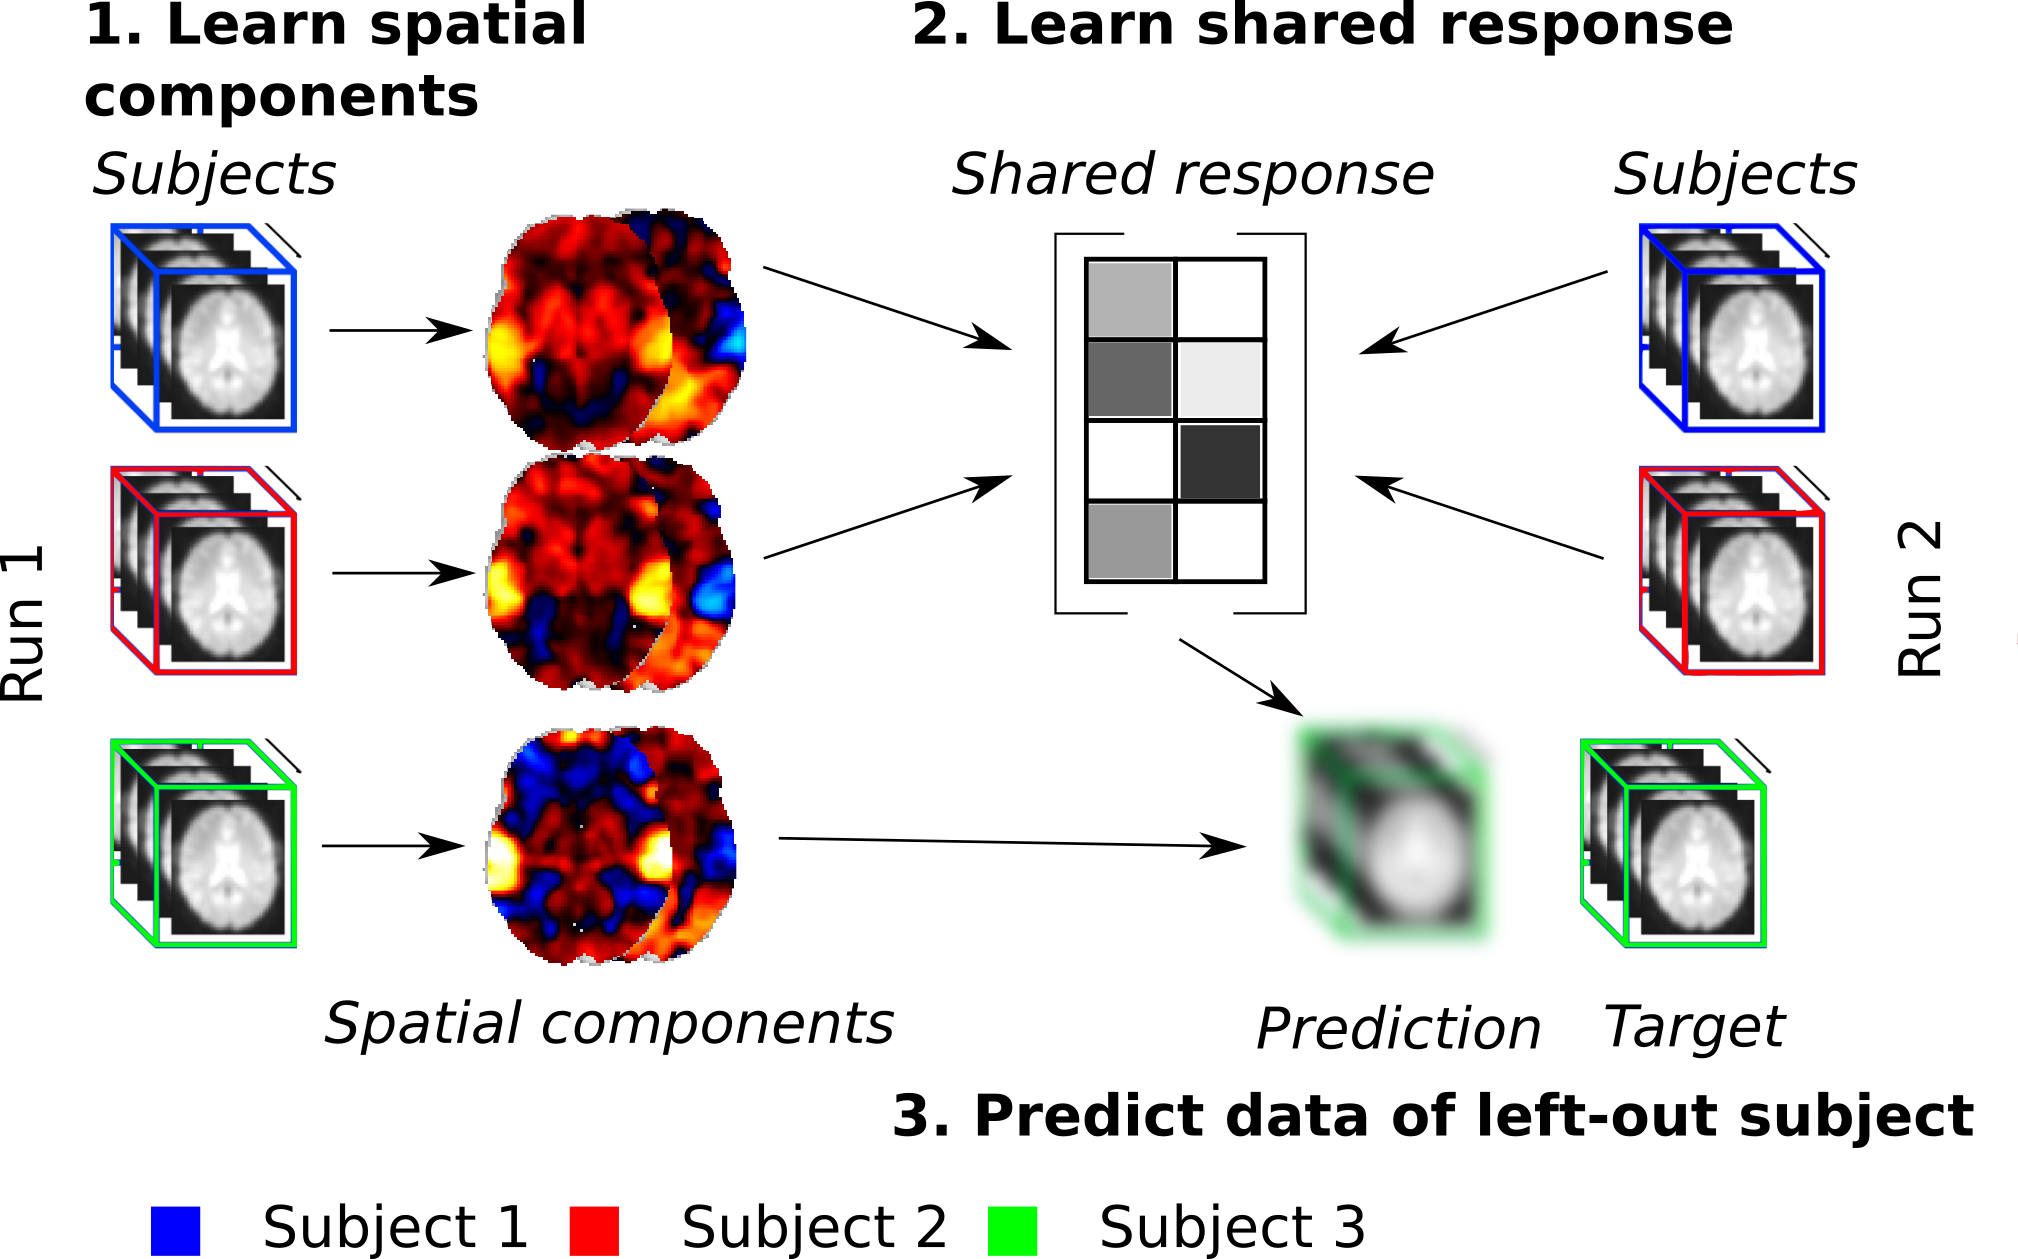
\includegraphics[scale=0.24]{figures/srm/conceptual_figure41.png}
\caption{\textbf{Experiment — Reconstruct data from a left-out subject} All runs but one are used to compute spatial components for every subject (left).
  %
  Then spatial components and data from the left-out run of all subjects but one are used to compute the shared response in the left-out run.
  %
  At last, the shared response during the left-out run and  the spatial components of the test subject are used to predict the data of the test subject in the left-out run.
  %
  The performance of the model is measured by comparing the prediction and true data using the $R^2$ score.}
\label{fig:experiment_reconstruction}
\end{figure}


An illustration of our reconstruction experiment is available in Figure~\ref{fig:experiment_reconstruction}.
%
The performance is measured voxel-wise using the $R^2$ score between $\widetilde{\mathbf{X}}_i^{(s)}$ and $\mathbf{X}_i^{(s)}$ as a similarity measure.
For any two time-courses $x \in \mathbb{R}^t$ and $y \in \mathbb{R}^t$ we define the $R^2$ score by:

\[
	R^2(x, y) = 1 - \frac{\sum_{z=1}^t (x[z] - y[z])^2}{\sum_{z=1}^t (y[z] - \overline{y}[z])^2} 
\]

Where $\overline{y} = \frac{1}{t}\sum_{z=1}^t y[z]$.
%
Following the leave-one-out cross validation scheme, all our experiments are done several times with a different left-out subject to reconstruct. 
%
We measure the average $R^2$ score across  all left-out subjects. Note that we obtain one such value per voxel.

\subsubsection{Predict age from spatial components}
Since spatial components are subject-specific they should be predictive of subject-specific features such as age.
%
In this experiment we try to predict subject's age from movie-watching data using SRM algorithms.
%
Functionally matched spatial components are obtained using an SRM algorithm.
%
They are divided into two groups (train and test data) where the train set contains 80\% of the data and the test set 20\%.
%
Within the train set we split again our data into two groups: the first group is used to train one Ridge model per spatial components, the second group is used to train a Random Forest to predict age from Ridge predictions. This way of stacking models is similar to the pipeline used in \cite{rahim2017joint}.
%
We use 5 fold cross validation to split the train set (so that the number of samples used to train the Random Forest is the number of elements in the train set).
%
Then the train set is used to train one Ridge model per spatial component.
%
On the test set each Ridge model makes a prediction and the predictions are aggregated using the Random Forest model.
%
An illustration of the process is available in Figure~\ref{fig:experiment_age_prediction}. 

In each Ridge model, the coefficient that determines the level of l2 penalization is set by generalized cross validation, an efficient form of leave-one-out cross validation (see the RidgeCV implementation of Scikit Learn \cite{pedregosa2011scikit}).

The train and test sets are chosen randomly. 5 different choices for the train and test set are made. We report the average mean absolute error (MAE) on the test set averaged over the 5 splits.

\begin{figure}
\centering
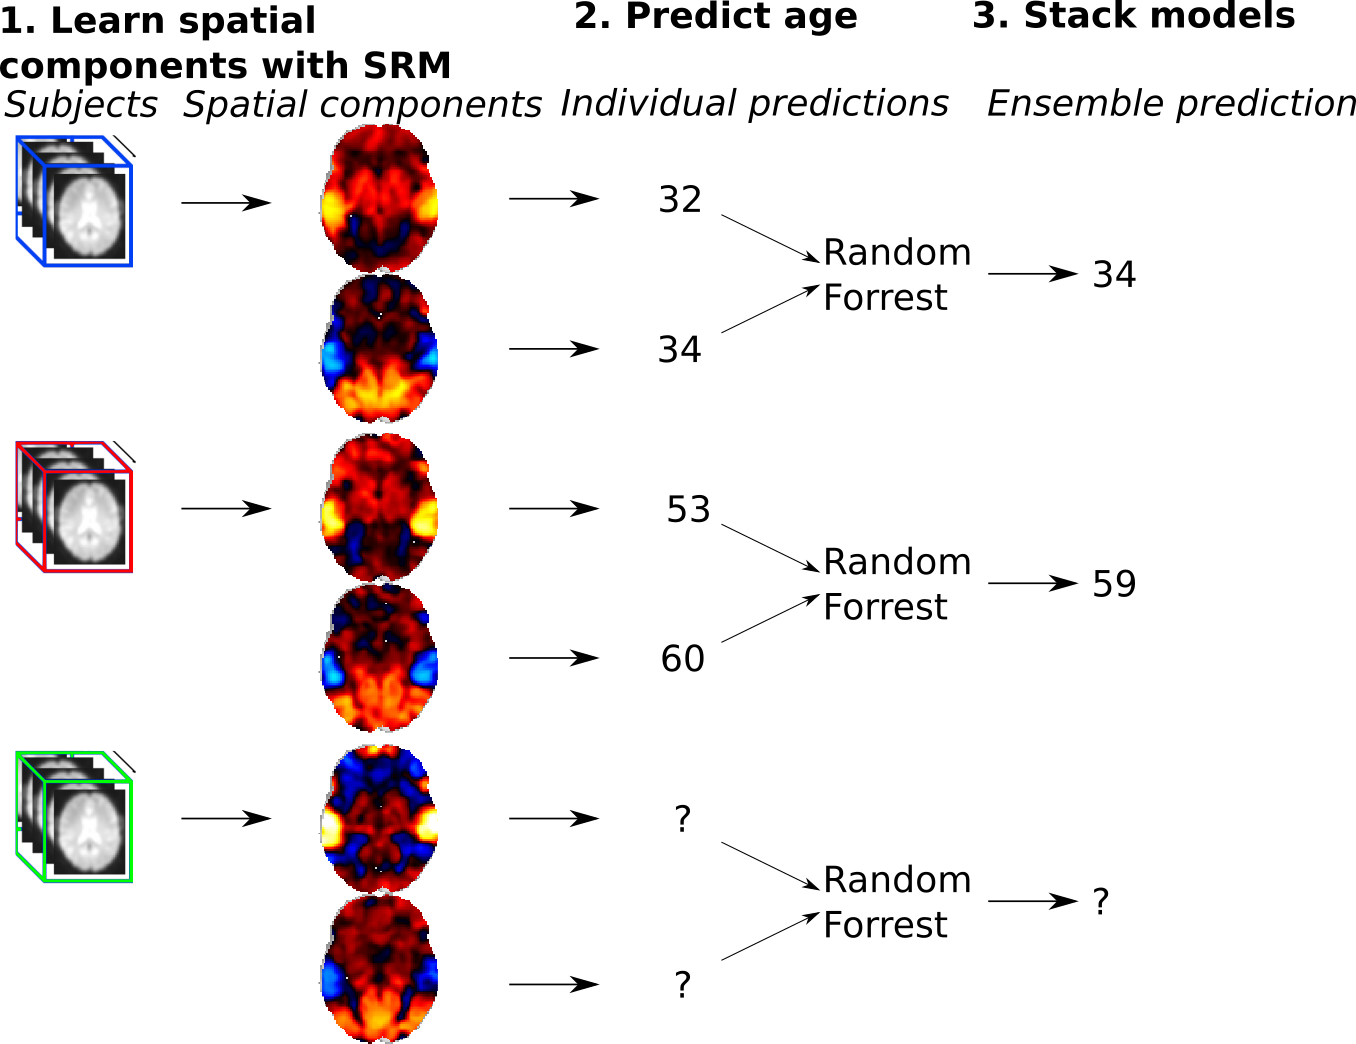
\includegraphics[scale=0.35]{figures/srm/conceptual_figure72.png}
\caption{\textbf{Experiment — Predict age from spatial components extracted using FastSRM}: We first learn the spatial components from fMRI data using SRM. We learn one Ridge model per spatial components to predict age across subjects. Then, these models are aggregated using a Random Forest (like in \cite{rahim2017joint}).} 
\label{fig:experiment_age_prediction}
\end{figure}


\section{Results and Discussion}

\subsection{fMRI Reconstruction}
We perform the reconstruction experiment on the FORREST, CLIPS, RAIDERS and SHERLOCK datasets. We compare brainiak's implementation of ProbSRM / DetSRM to our implementation of FastSRM in terms of fitting time, memory usage and performance. In order to be fair, we do not use parallelization ($n_{jobs} = 1$) and we set the number of iterations to 10 ($n_{iter}=10$) which is ProbSRM's default. Note that the fitting time of ProbSRM is roughly proportional to the number of iterations while it has a limited impact on the fitting time of FastSRM. 


We run our experiments on the full brain and report an $R^2$ score per voxel.
%
However we measure the performance in terms of mean $R^2$ score inside a region of interest (in order to leave out regions where there is no useful information).
%
In order to determine the region of interest, we focus on the results of ProbSRM with $10, 20, 50$ and $100$ components and keep only the intersection of regions where the $R^2$ score is above $0.05$.
%
This means of selecting regions favors ProbSRM. For completeness, full brain $R^2$ images obtained on the four datasets with ProbSRM and FastSRM using $20$ components averaged across subjects are available in Figure~\ref{fig:example_r2}.

In Figure~\ref{fig:mean_r2_score}, we plotted the mean $R^2$ score against the number of components ($k$) for ProbSRM, DetSRM and FastSRM algorithm with different atlases.
%
The $R^2$ score tends to increase with the number of components (which is what is expected as more information can be retrieved when the number of components is high).
%
FastSRM matches the performance of ProbSRM and DetSRM. This holds for any atlas we chose (BASC (444 parcels), SHAEFFER (800 parcels), MODL (512 and 1024 parcels)) and for all datasets we tried (SHERLOCK, RAIDERS, CLIPS and FORREST). 

In Figure~\ref{fig:fit_time}, we compare the running time of FastSRM, DetSRM and ProbSRM on the four different datasets.
%
FastSRM is on average (across datasets) about 5 times faster.
%
On the FORREST dataset, we compute a shared response in about 3 minutes when it takes about 20 minutes with ProbSRM or DetSRM.

In Figure~\ref{fig:memory_usage}, we compare the memory (RAM) consumption of FastSRM, DetSRM and ProbSRM on the four different datasets.
%
FastSRM is 20 to 40 times more memory friendly than ProbSRM and 10 to 20 times more memory friendly than DetSRM. On the FORREST dataset the memory usage of FastSRM is between 1 and 3 Go depending on the number of components and the atlas used. Most modern laptops meet these requirements. On the same dataset memory consumption is about 80 Go for ProbSRM and 40 Go for DetSRM which is manageable but costly for small labs.
%
Overall FastSRM yields same performance as ProbSRM and DetSRM while being much faster and using far less memory. We also show that the atlas used to reduce the data only has a minor impact on performance.

\begin{figure}
\centering
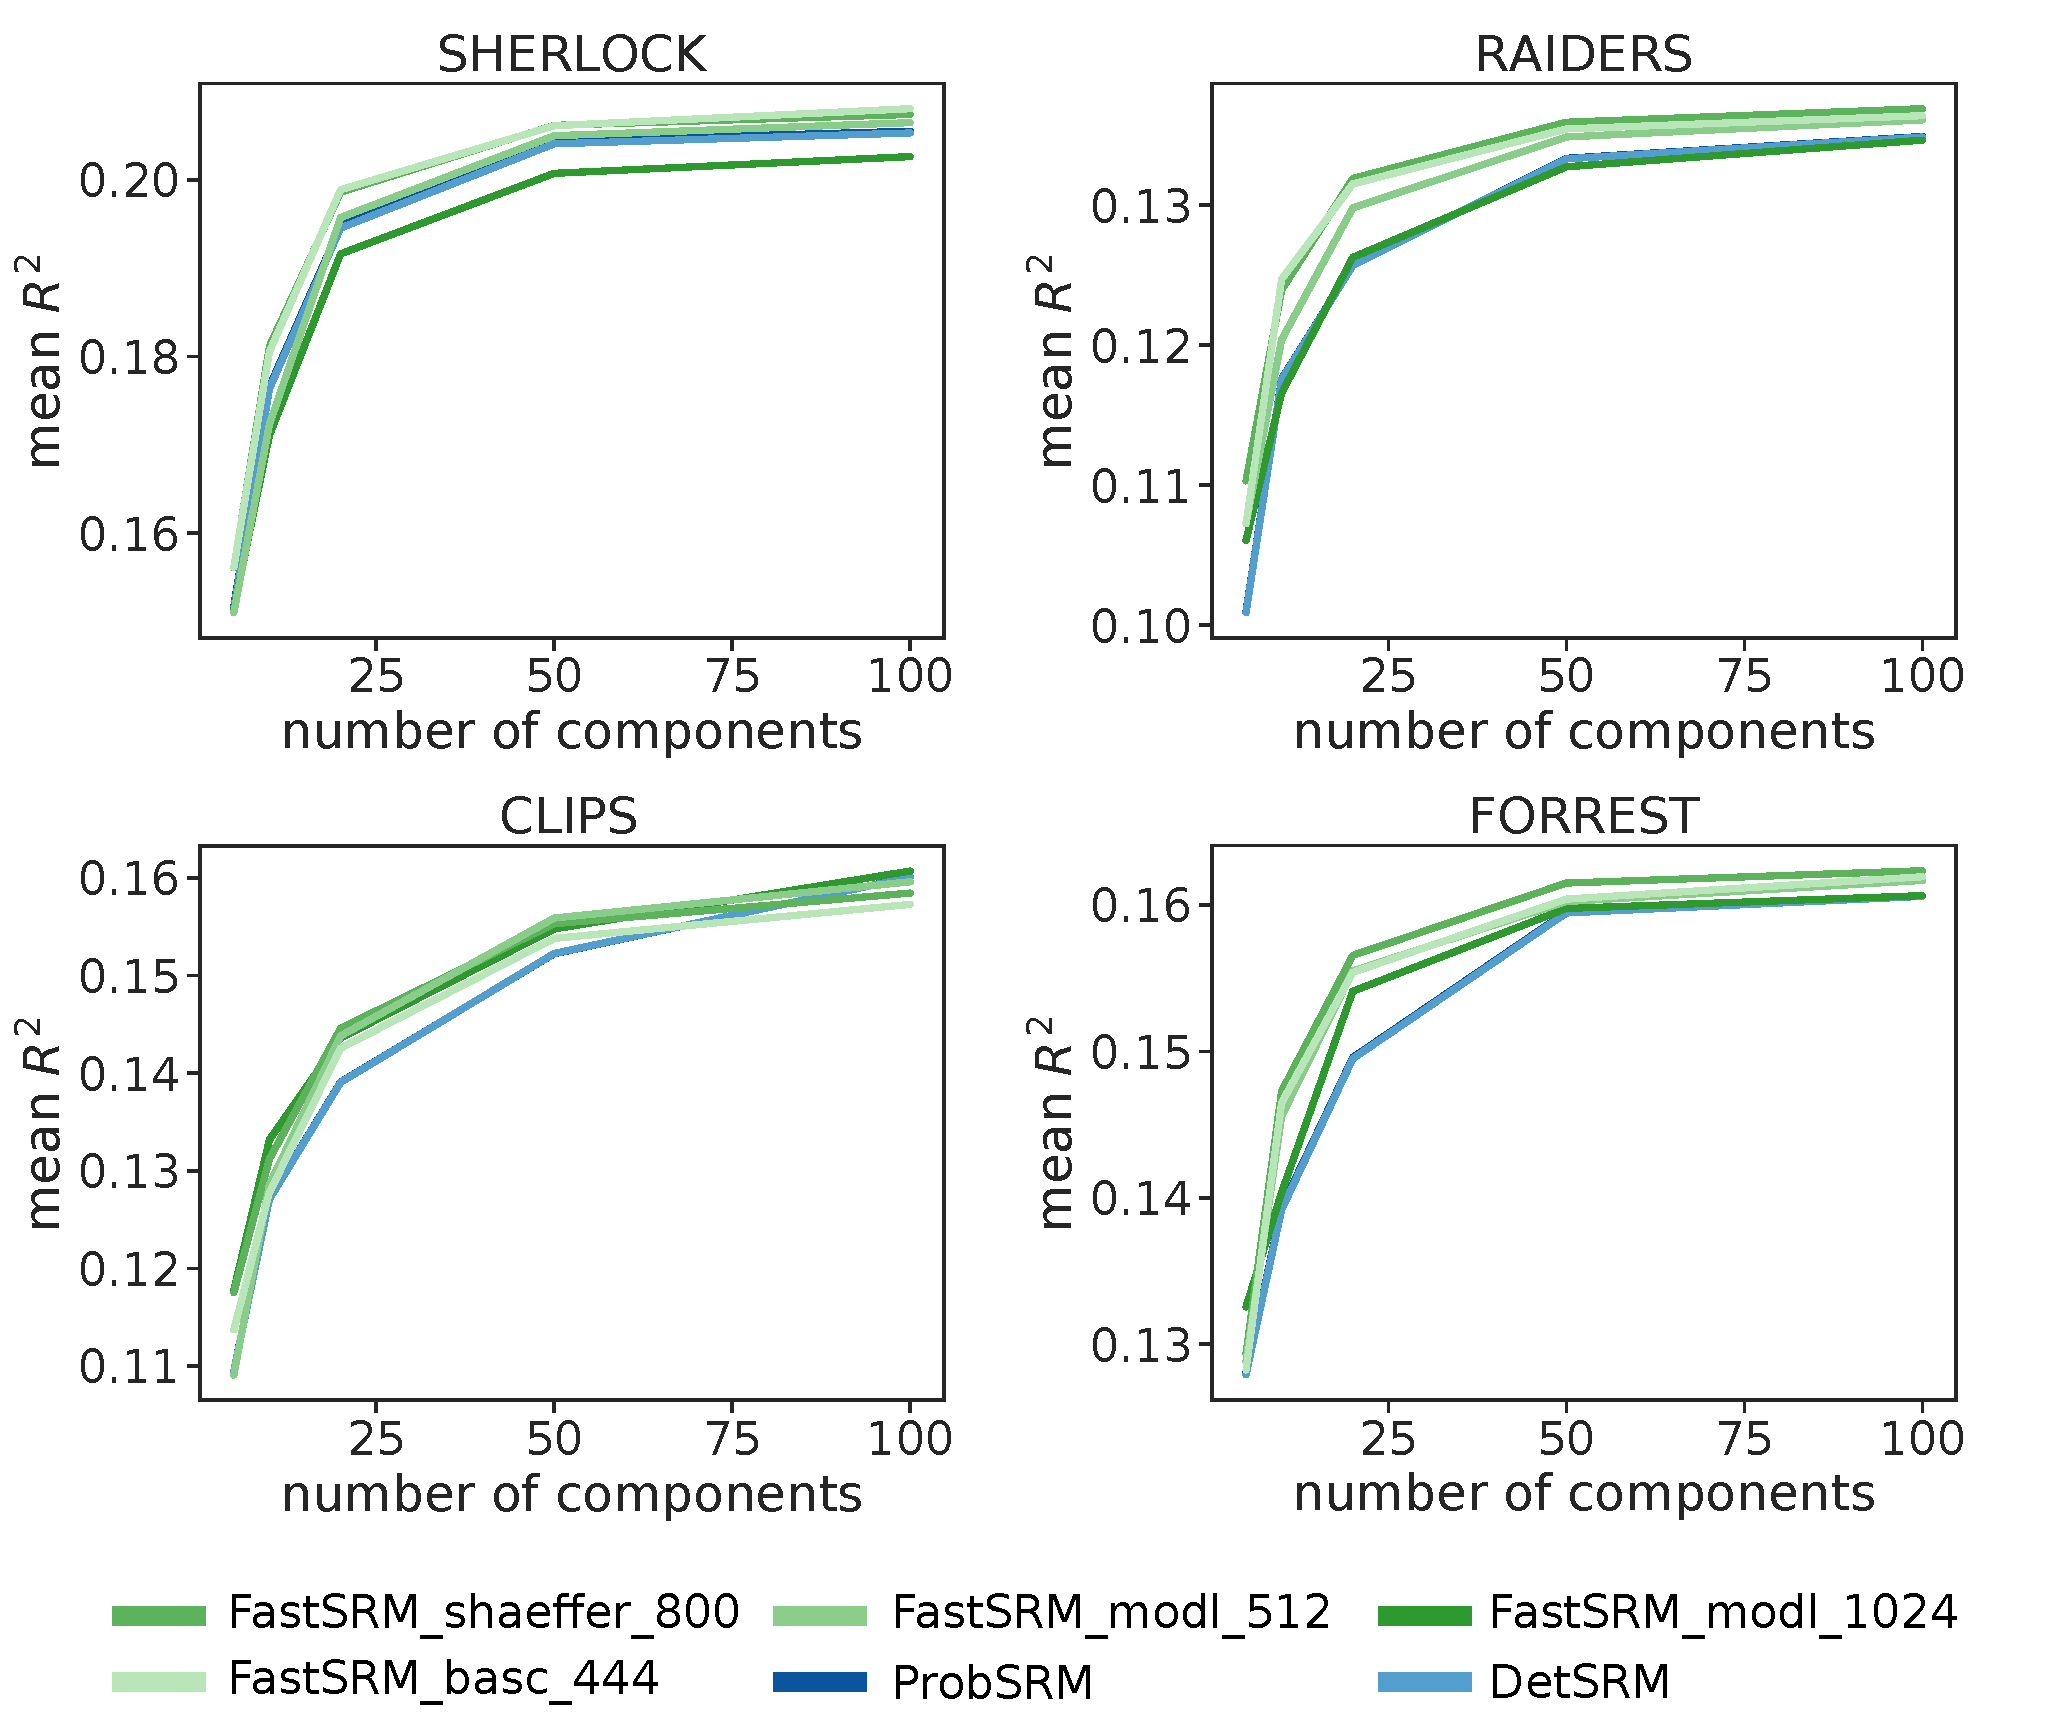
\includegraphics[scale=0.34]{figures/srm/perfs.pdf}
\caption{\textbf{Performance of the methods in an encoding test} We compare the performance (measured in terms of average $R^2$ score in a region of interest) of ProbSRM and FastSRM with different atlases in function of the number of components used. Atlases tested are MODL with 512 and 1024 parcels, Basc with 444 parcels and Shaeffer with 800 parcels. Datasets tested are SHERLOCK (top left), RAIDERS (top right), CLIPS (bottom left) and FORREST (bottom right). 
As we can see, no matter which atlas is chosen, FastSRM matches ProbSRM's performance.}
\label{fig:mean_r2_score}
\end{figure}

\begin{figure}
\centering
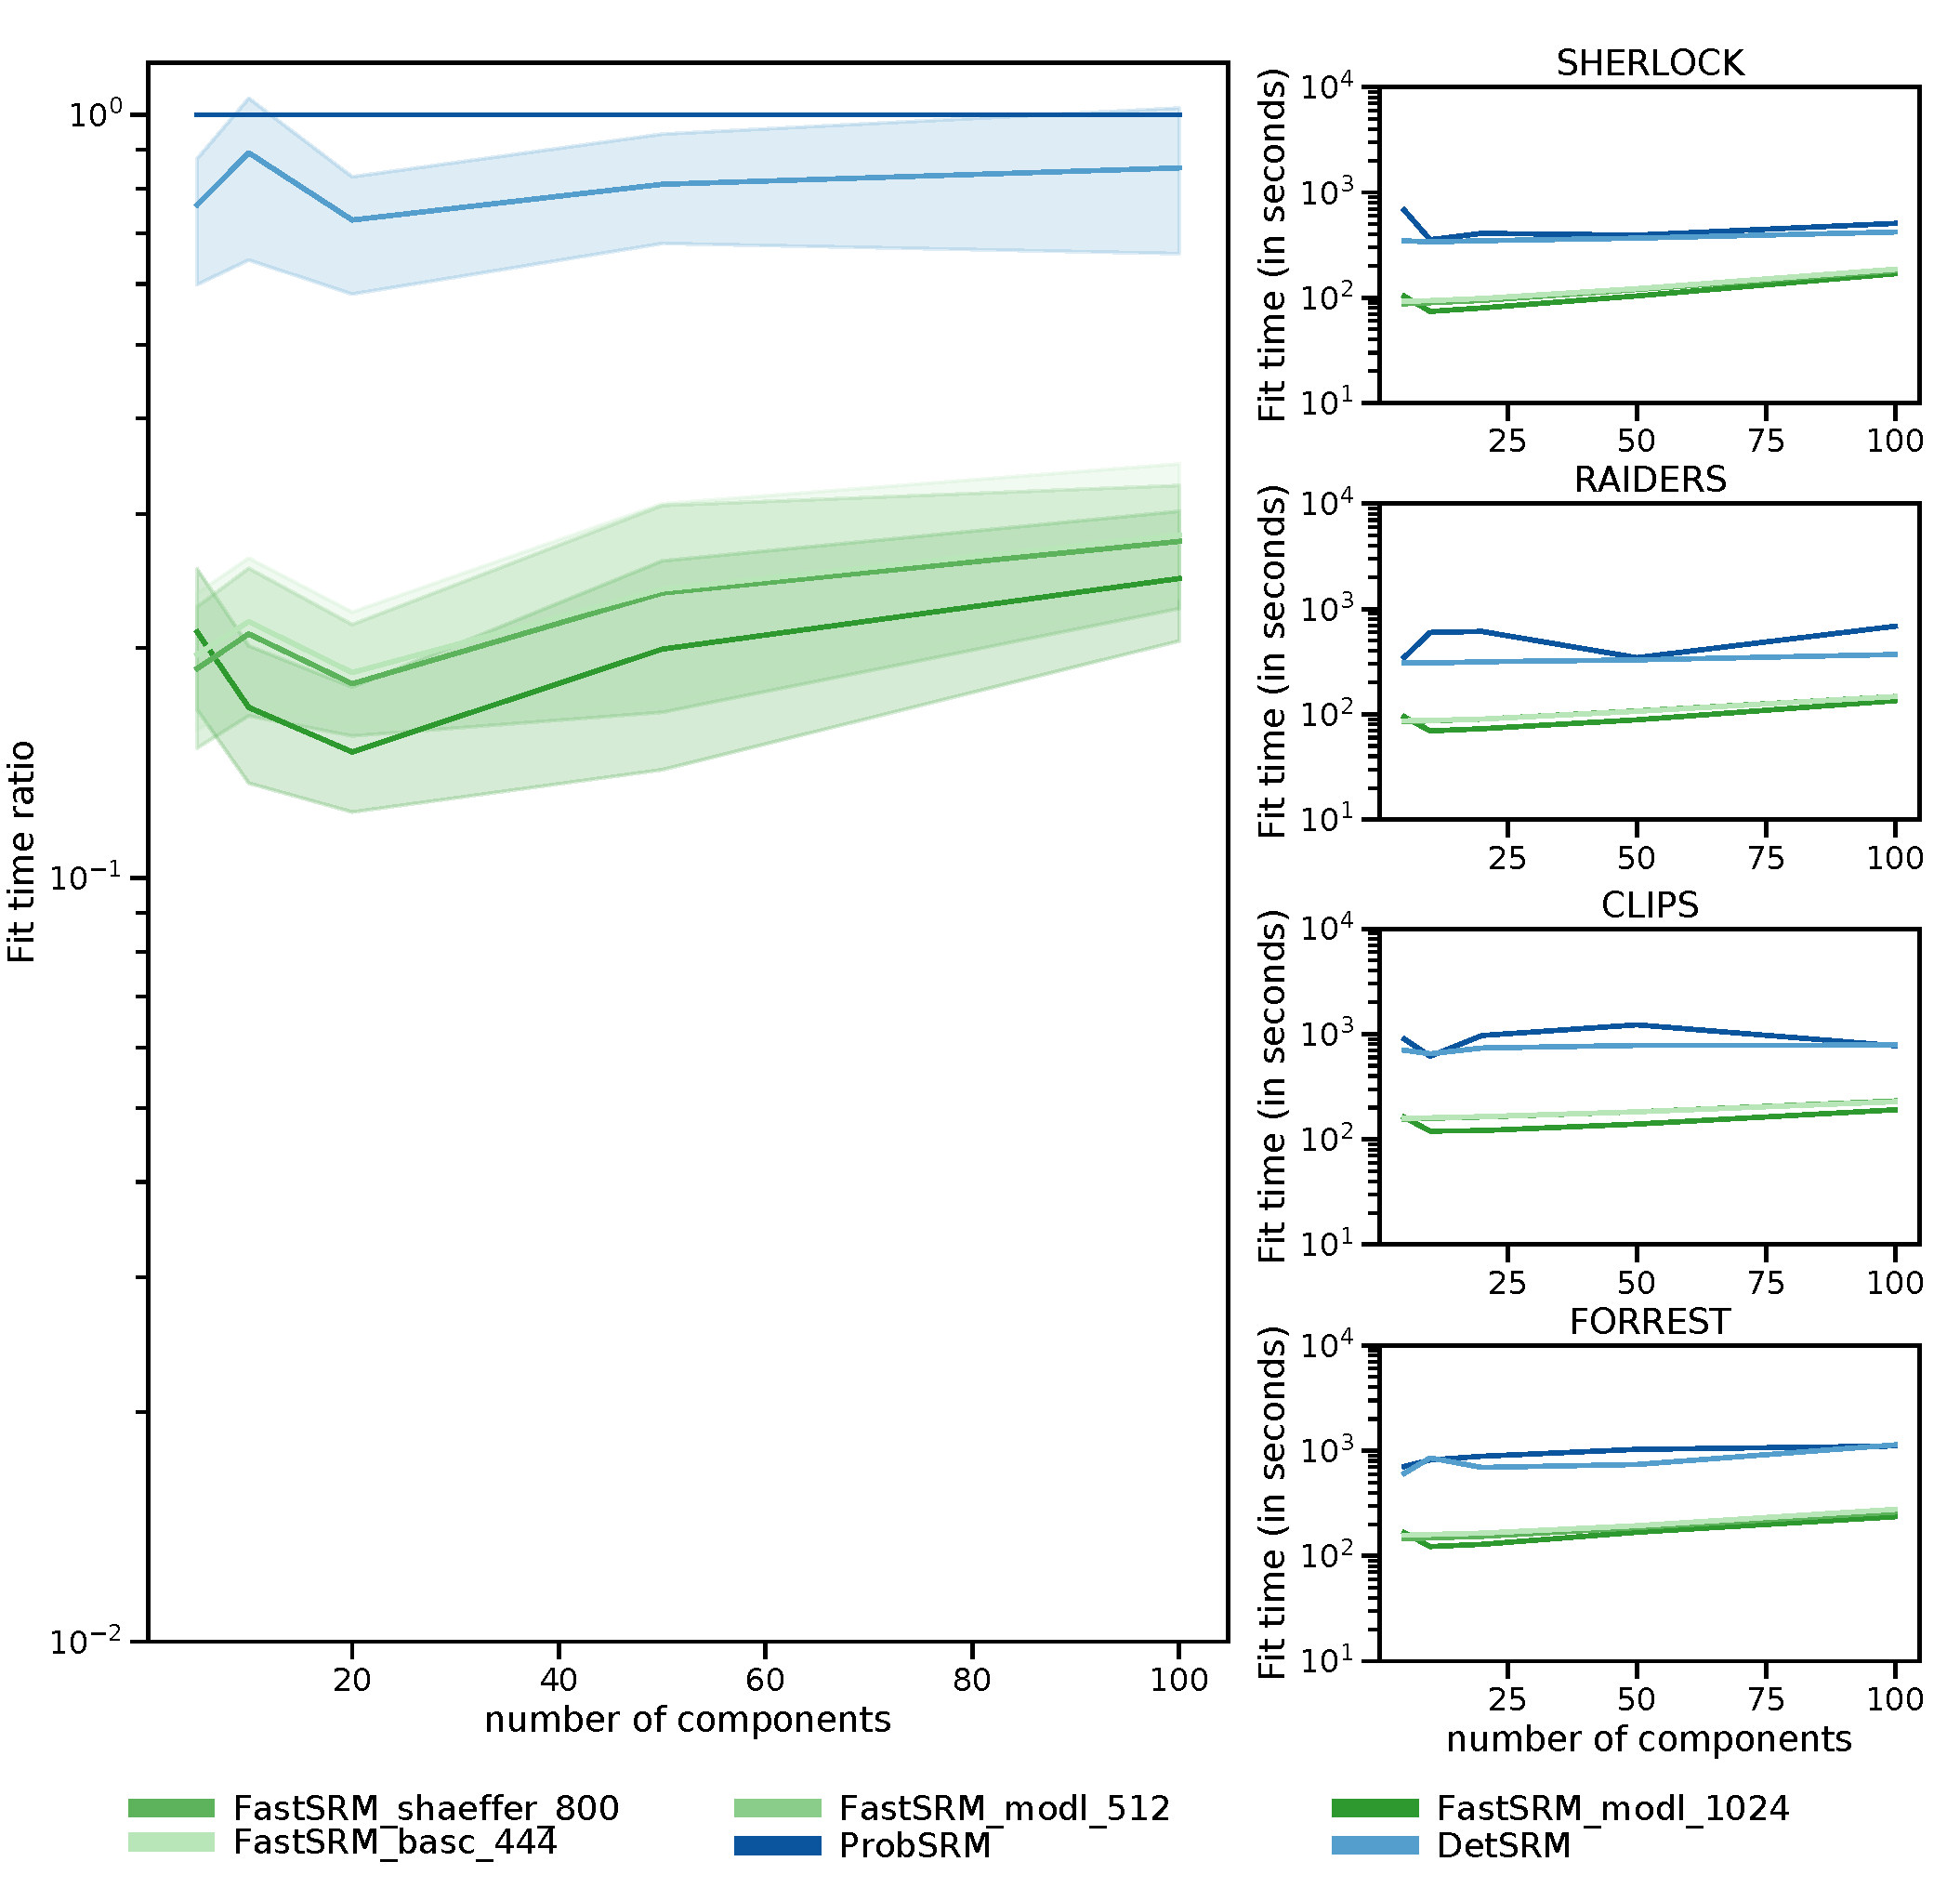
\includegraphics[scale=0.33]{figures/srm/fit_time.pdf}

\caption{\textbf{Fitting time of FastSRM, ProbSRM and DetSRM} We compare the fitting time of ProbSRM, DetSRM and FastSRM with different atlases in function of the number of components used. Atlases tested are MODL with 512 and 1024 parcels, Basc with 444 parcels and Shaeffer with 800 parcels. Datasets tested are SHERLOCK, RAIDERS, CLIPS and FORREST.
\textbf{Left}: Fitting time (as a fraction of ProbSRM fitting time) averaged over the four datasets.
\textbf{Right}: Fitting time (in seconds) for each of the four different datasets.
FastSRM is about 5 times faster than ProbSRM.}
\label{fig:fit_time}
\end{figure}

\subsection{Predicting age from spatial components}
Because FastSRM is fast and memory efficient, it enables large-scale analysis of fMRI recordings of subjects exposed to the same naturalistic stimuli.
%
We use all 647 subjects of the CamCAN dataset and demonstrate the usefulness of FastSRM by showing that the spatial components it extracts from movie watching data are predictive of age.
%
A key asset of FastSRM is that these spatial components can be visualized and therefore provide meaningful insights. 

Figure~\ref{fig:predict_age} shows that FastSRM predicts age with a good accuracy (better than ProbSRM and a lot better than chance) resulting in a mean absolute error (MAE) of 7.5 years.
%
It also shows that on CamCAN data, FastSRM is 4x faster and more than 150x more memory efficient than ProbSRM. As before and in order to ensure fair comparison the number of iterations is set to $10$ and we do not make use of parallelization. Note that the memory requirements of ProbSRM on the CamCAN dataset (186Go) make it difficult to use.
%
FastSRM does not suffer from memory issues, making it suitable to analyse big datasets.

A key asset of our pipeline is that we can see which spatial components are most predictive of age by using feature importance.
%
Feature importance is assessed by the Gini importance defined in \cite{breiman2001random} or \cite{louppe2013understanding}.
%
It measures for each feature the relative reduction in Gini impurity brought by this feature.
%
Feature importance varies with different splits. We use the averaged feature importance over the 5 splits of our pipeline.
%
In Figure~\ref{fig:predict_age} are shown the 3 most important spatial components representing respectively 16\%, 12\% and 8\% of total feature importance.
%
These spatial components in decreasing order of importance represent the visual dorsal pathway, the precuneus and the visual ventral pathway. 
%
The fact that averaged spatial components are interpretable and meaningful allows us to study the influence of age on brain networks involved in movie-watching.
%
In Figure~\ref{fig:predict_age_interpretation}, we plot the most important spatial component averaged within groups of ages.
%
We see that these spatial components evolve with age allowing us to visually identify which regions are meaningful. 
%
It turns out that aging is mostly reflected in brain activity as a
fading of activity in the spatial correlates of movie watching,
particularly in the dorsal visual cortex.
%
%With FastSRM, we can see how networks involved in movie-watching evolve with age. 


\begin{figure}
\centering
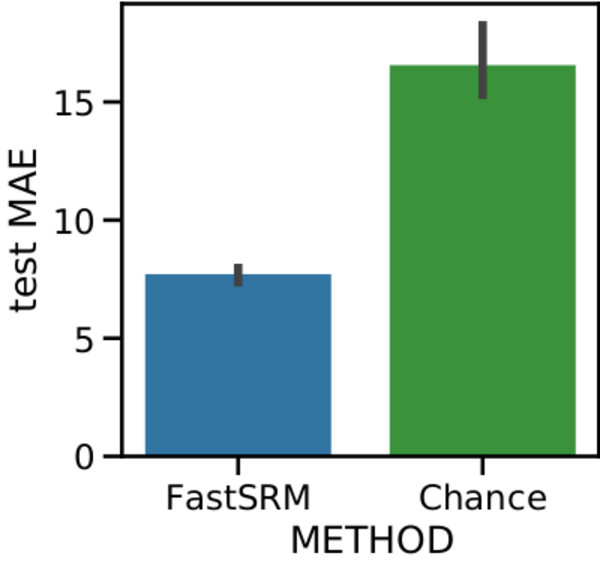
\includegraphics[scale=0.44]{figures/srm/predict_age.pdf}

\begin{tabular}{|c|c|c|}
	\hline
	Algorithm & Memory usage (in Go) & Fitting time (in minutes) \\
	\hline
	FastSRM & 1.1 & 15 \\
	ProbSRM & 186.3 & 69 \\
	\hline
\end{tabular}
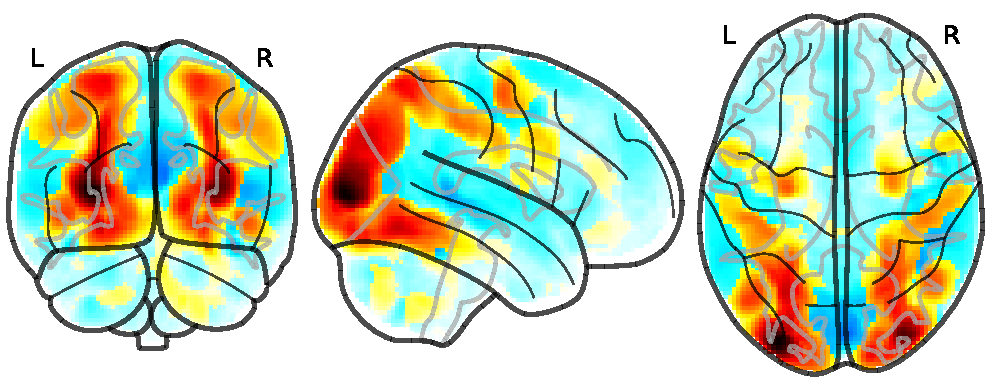
\includegraphics[scale=0.365]{./figures/srm/maps_feature_imp_0_16.pdf}
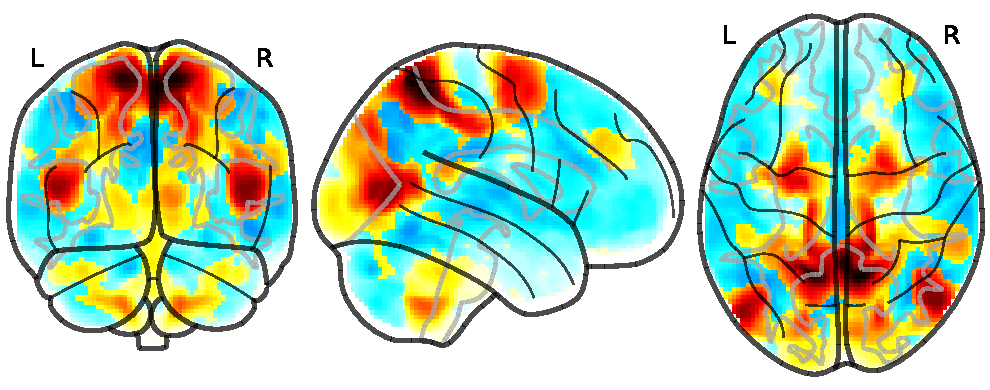
\includegraphics[scale=0.365]{./figures/srm/maps_feature_imp_0_12.pdf}
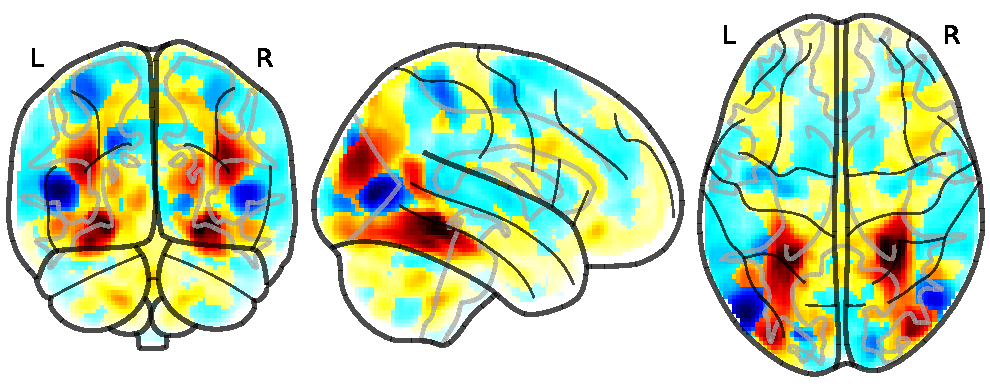
\includegraphics[scale=0.365]{./figures/srm/maps_feature_imp_0_08.pdf}

\caption{\textbf{Age prediction from spatial components}: (top) FastSRM predicts age with a good accuracy (better than ProbSRM and a lot better than chance) resulting in a mean absolute error (MAE) of 7.5 years. (middle) FastSRM is more than 4x faster than ProbSRM and uses 150x less memory, hence it scales better than ProbSRM. (bottom) The three most important spatial components in terms of the reduction in Gini impurity they bring (see Gini importance or Feature importance in \cite{breiman2001random}, \cite{louppe2013understanding}). From top to bottom, the most important spatial component (feature importance: 16\%) highlights the visual dorsal pathway, the second most important spatial component (feature importance: 12\%) highlights the precuneus and the third most important spatial component (feature importance: 8\%) highlights the visual ventral pathway.} 
\label{fig:predict_age}
\end{figure}

\begin{figure}
\centering
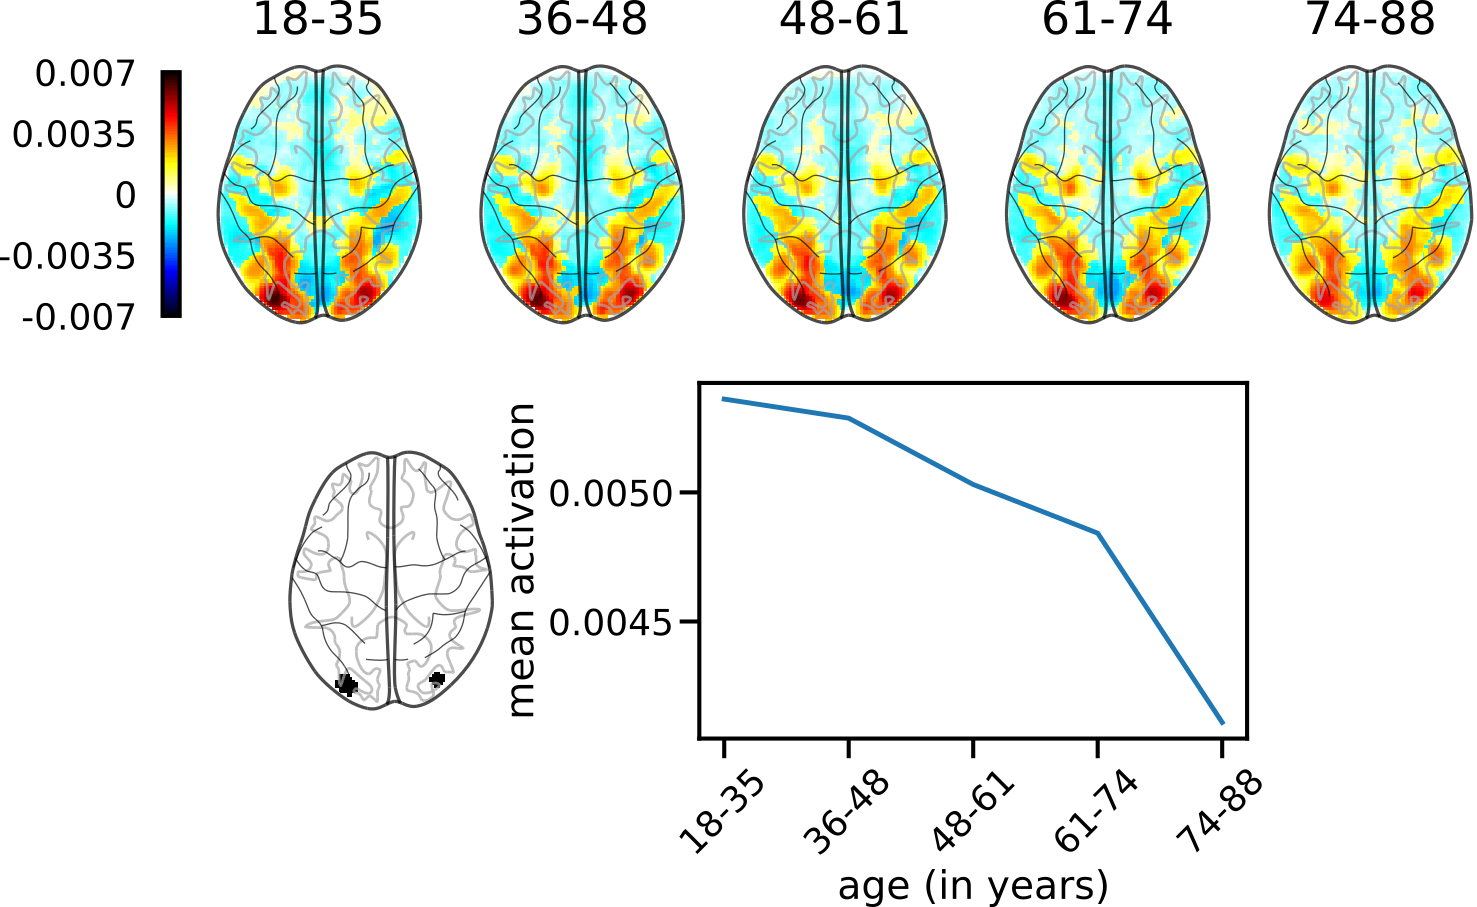
\includegraphics[scale=0.35]{figures/srm/feature_importance_age_prediction.png}
\caption{\textbf{Evolution of the most predictive spatial component with age}: (Top) Spatial component most predictive of age averaged within groups of different age (18-35, 36-48, 48-61, 61-74, 74-88). (Bottom) Mean activation in the region highlighted by the mask on the left. We see that the activity in the dorsal pathway decreases with age, which explains why this spatial component is a good predictor of age.}
\label{fig:predict_age_interpretation}
\end{figure}



\subsection{Conclusion}
As studies using naturalistic stimuli will tend to become more common and large within and across subjects, we need scalable models especially in terms of memory usage.
%
This is what FastSRM provides.
%
We show that while FastSRM matches the performance of ProbSRM or DetSRM, it is
significantly faster and requires a lot less memory. While FastSRM's scalability relies on the use of atlases to compress the BOLD signal, we show that the precise choice of the atlas has only marginal effects on performance.


FastSRM allows large scale analysis of fMRI data of subjects exposed to naturalistic stimuli. As one example of such analysis, we show that it can be used to predict age from movie-watching data. Interestingly, although FastSRM is an unsupervised model, it extracts meaningful networks and as such constitutes a practical way of studying subjects exposed to naturalistic stimuli.

We also show that individual information can be extracted from the fMRI activity when subjects are exposed to naturalistic stimuli. Our predictive model is reminiscent of that of \cite{bijsterbosch2018relationship}, that have shown that ICA components obtained from the decomposition of resting state data carry important information on individual characteristics. 
%

As a side note, we chose to keep the orthonormality assumptions of the original SRM model but slight modifications of our implementation of FastSRM would allow one to build more refined model promoting sparsity, non-negativity or smoothness of spatial components for example.

The remaining difficulty with SRM is to interpret the spatio-temporal decomposition. Reverse correlation \cite{hasson2004intersubject} can be used to clarify the cognitive information captured in the shared response.

Our code is freely available at \url{https://github.com/hugorichard/brainiak/tree/fastsrm}.

